\documentclass[12pt]{ociamthesis}  % default square logo 
%\documentclass[12pt,beltcrest]{ociamthesis} % use old belt crest logo
%\documentclass[12pt,shieldcrest]{ociamthesis} % use older shield crest logo

%load any additional packages
\usepackage{amssymb}

%input macros (i.e. write your own macros file called mymacros.tex 
%and uncomment the next line)
%\include{mymacros}

\title{EEG ANALYSIS OF DRUG USERS WITH WAVELET METHODS \\[3ex]     %your thesis title,
        Internship I}   %note \\[1ex] is a line break in the title

\author{Daniel Septry Panjaitan}             %your name 
\college{1.14.4.085\\[5ex]
In Partial Fulfilment of The Requirements for 
The Degree of Applied Bachelor of Informatics Engineering}  %your college

%\renewcommand{\submittedtext}{change the default text here if needed}
\degree{Politeknik Pos Indonesia}     %the degree
\degreedate{Bandung 2018}         %the degree date

%end the preamble and start the document
\begin{document}

%this baselineskip gives sufficient line spacing for an examiner to easily
%markup the thesis with comments
\baselineskip=12pt plus1pt

%set the number of sectioning levels that get number and appear in the contents
\setcounter{secnumdepth}{3}
\setcounter{tocdepth}{3}


\maketitle                  % create a title page from the preamble info
\begin{dedication}
`Jika Kamu tidak dapat menahan lelahnya belajar, \\
Maka kamu harus sanggup menahan perihnya Kebodohan.'\\ 
~Imam Syafi'i~\\
\end{dedication}        % include a dedication.tex file
\begin{acknowledgements}
All praise and gratitude writer are turning to the presence of God Almighty because with His bounties and blessings I can finish first Internship report titled "Analysis of EEG Against Drug Users Using WAVELET Method" which is one of the requirements to continue the learning process to the next level. 
\par
In writing this, I Internship report writers face many obstacles, one of which is the difficulty in obtaining data and information as well as the limitations of the knowledge possessed by the author. However, the authors attempted with the capabilities to complete this report.
\par
For that on this occasion the author would like to thank:

\begin{enumerate}
    \item To Parents, Brothers, and All my friends who have supported both regarding morale to the material.
    \item Both my parents and family have encouraged and encouraged me.
    \item Rolly Maulana Awangga, ST, MT as lecturers on campus and in the Internship which has provided guidance as well as ease of analysis and preparation of reports.
    \item All those who have contributed to the completion of this first Internship report.
    \item Syafrial Fachri Pane, S.T., M.T.I. As the Companion Examiner for this Internship I stage.
    \item Roni Andarsyah. S.T., M.Kom. As Internship I Coordinator for Academic Year 2018/2019.
    \item M. Yusril Helmi Setyawan, S.Kom., M.Kom. As Chair of the 2018/2019 DIV Informatics Engineering Study Program.
    \end{enumerate}
\par
The author realized that writing this report is far from perfect, therefore, criticism and constructive suggestions are needed by the author to work more leverage for the future. 
\par
End the authors hope that this report can be useful and add a better insight to the reader. 

\par
\begin{raggedleft}
Bandung, december 11, 2018

\end{raggedleft}


\end{acknowledgements}

   % include an acknowledgements.tex file
\begin{abstract}
\textit{\indent
% Text of abstract
Electroensephalogram (EEG) is an activity to record the electrical activity of brain neurons. EEG is often used to analyze brain activity and predict the emotions produced, by using EEG relaxed conditions of drug users can be observed. EEG signals are widely used to detect brain disorders in the health world. However, the signal produced by the EEG needs to be prepared for the process to be able to detect brain abnormalities automatically. Therefore, there is a need for a preprocessing method to produce the right features in order to obtain precisely and accurately stored characteristics of the EEG signal. This research will be developed using the Loreta method. Therefore, the researcher will design portable devices and application systems that can monitor the condition of the brain using EEG sensors correctly.
	%%
	}
\end{abstract}
          % include the abstract

\begin{romanpages}          % start roman page numbering
\tableofcontents            % generate and include a table of contents
\listoffigures              % generate and include a list of figures
\listoftables
\end{romanpages}            % end roman page numbering

%now include the files of latex for each of the chapters etc
\chapter{Introduction}
\section{Background}
Drug broadcasting among youth and teenagers cannot be denied and still consume it in the environment around us. It seems to be for health and a little future. \cite{wagner2016using}
\par
The danger of drugs for addicts and adolescents, students is very much and if not immediately spent on buying drugs then drug use will overdose and one of the factors that can be felt from drug use can damage the mental and cure the tragic. \cite{warnock2018life}
\par
The effect parameters derived from quantitative EEG analysis seem to be very suitable for marking relationships between nakoba users or not drug users. EEG parameters represent many characteristics of pharmacodynamic actions that are ideal, sustainable, and objective These features provide an opportunity to find out the relationship between the effects for drugs on individuals, which makes valuable information about brain waves of drug users.\cite{mandema1992electroencephalogram}
\par
 Electroencephalogram (EEG) is an activity to record the electrical activity of brain neurons. EEG is being used.\cite{hanley2017brain} Using EEG, the condition of relaxing or not drug users can be observed. EEG signals are widely used to detect brain disorders in the world of health. However, EEG signals are not made to be ready to detect brain abnormalities automatically. Therefore, the characteristics of the EEG signal are safe.\cite{zotev2018real} Simultaneous EEG modulation of the volume of BOLD activity from the target brain region and investigation of electrophysiological activities related to the results of objects using illegal drugs will show human brain waves.\cite{chiang2017dangers} electroencephalography (EEG), we investigated and compared reciprocal accuracy and efficiency and direct EEG forward approaches for brain electrical current sources based on existing methods, adjoint (AA) approaches and partial integration approaches in relation to the concept of data transfer matrices. By analyzing numerical results, comparing with EEG's advanced potential is derived analytically and estimates complexity. \cite{palva2018ghost}, and to overcome the effects of linear sources attached to standard interaction steps, alternative phases and connectivity steps based on amplitude correlations, such as imaginary coherence and orthogonal amplitude correlations proposed. Defined to be insensitive to zero-lag correlation, this technique has become increasingly popular in the identification of correlations that cannot be attributed to field spread or volume conduction. This fundamental problem is region-based analysis and importance-for-all mapping. Most importantly, beyond defining and describing the problem of false interactions, we provide strict quantification of these effects through extensive simulations. In addition, we further demonstrated that the mixing signal also limits the separation of the neuron phase and amplitude correlation
 \par
 Methadone is a type of synthetic opioid drug, used as an analgesic and for treating addiction from users of the opioid group, such as heroin, morphine, and codeine. But its improper use can also have a negative impact on health. Although methadone is indispensable for medical treatment and services, especially drug addicts, if it is misused or used is not by the standard of treatment, especially if accompanied by illicit circulation, it will have a very detrimental e ect on individuals or society ,especially the younger generation. \cite{lim2015analysis} Detection of the use of methadone and other types of drugs is quite a lot done in government agencies, hospitals, and industries to screen employees/workers who will carry out medical tests. Already many methods used are detection using urine, using saliva or doing screening by doing brain signal recording. \cite{jin2015p300}
\section{Problems Identification}
Identify the problem based on the background are:
\begin{enumerate}
    \item How the human brain wave monitor for drug users
\end{enumerate}

\section{Objective and Contribution}
\subsection{Objective}
\begin{enumerate}
    \item Monitoring the human brain waves against drug users
\end{enumerate}
\subsection{Contributione}
\begin{enumerate}
    \item Help monitor brain waves to drug users and the detection of EEG signals
\end{enumerate}
\section{Scoop and Environtment}
The scope of the study conducted by researchers are:
\begin{enumerate}
    \item Showing graph EEG
    \item Real-Time Monitoring brain waves and determine the characteristics based  on the EEG signals. 
\end{enumerate}
\chapter{Related Works}

\section{Electroencephalogram}
Elektroensefalografi(EEG) is a test that is widely used to detect brain waves. This signal is recorded by the deviceElectroencephalography, Is hardware that functions record the electrical activity of a brainwave. The working principle of this EEG detects activity electricity from the brains of people with that recorded by silver electrodes that are installed by trained technicians in the scalp. In this study, participants brain activity was observed using an electroencephalogram (EEG) while each of the participants completed spatial ability assessments\cite{ruesch2017understanding}
\par
The medical community using EEG, among others for the diagnosis of diseases associated with the brain and psychiatric disorders. EEG is also applied to detect patterns of mind or mental condition of a person. Visual observation of the EEG signal directly is challenging given the EEG signal amplitude is low and thus a very intricate pattern. Besides, the EEG signals are strongly influenced by a variety of variables, such as mental state, health, the activity of the patient, the recording environment, electrical interference from other organs such external stimuli, and the age of the patient. The nature of EEG signals is generally non-stationary and random, so that adds to the complexity in the processing of EEG signals. However,\cite{perry2017effects}

\section{Brain}
The brain is a central nervous system consisting of billions of cells called neurons. Each neuron communicates with each other and emits electric waves or commonly known as brain waves. Brain waves can be measured using an electroencephalogram (EEG). Brain waves produce frequencies that vary between 0.5-30 Hz and are classified into delta, theta, alpha, and beta waves. Each stream has different characteristics and shows a person's mental state. where every brain activity is very dependent on the situation of drug users, and where loyal users must be the brain waves produced vary between brain waves produced by the drug user, and where the state of the brain mostly produces internal rhythms from outside the user's drug awareness.\cite{mccormick2015brain}

\subsection{Brain Waves}
Brain waves can be measured with equipment Electroencephalograph (EEG). It is known that the frequency of brain waves generated by neurons varies between 0-30 Hz and is classified into a delta wave, theta, alpha, and beta. Each stream has different characteristics and indicate a person's mental condition. Human brain waves have different frequency and amplitude range – different\cite{liu2015plasticity}, so it is divided into several types of waves as follows:

\begin{enumerate}
    \item Delta waves
    \par
   Delta waves have frequency waves that are worth 1.5 <4 Hz. Delta waves are one of the slowest waves of other brain waves, in this condition a person's body carries out a process of self-healing, repairing damage to body tissues, and actively producing new cells when a person is sound asleep\cite{assenza2015wakefulness}
   
    \item Theta waves
    \par
    Theta waveform has a frequency value between 4 -8 Hz with a voltage amplitude reaches 10 μV. These waves are generated when a person is experiencing light sleep or drowsiness\cite{chiu2015complexity}
    
    \item Alpha waves
    \par
   Alpha waves have a frequency value between 8-13 Hz, where this frequency is a control of the body or conscious and subconscious mind where a person can remember a dream or more significantly someone does meditation (mild meditation)\cite{okumura2006amplitude}
   
    \item Beta waves
    \par
   Types Beta waves have a frequency of between 14-19 Hz and 20-30 Hz in beta waves indicating that a person is experiencing mental wakefulness or someone can control himself or think that he is tired because a lot of work presses or complicated problem solving\cite{malik2018brain}
   
    \item Gamma waves
    \par
    Gamma waveforms have a frequency value of 30-40 Hz. These waves are produced when someone experiences extraordinary mental activity or can be said to be bad usually someone who is undergoing a match, is panicking or is scared\cite{martini2018spatial}
    
    \begin{figure}[h!]
\centering
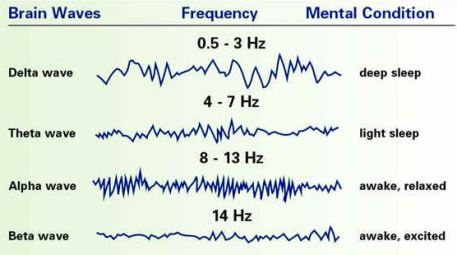
\includegraphics[scale=0.6]{figures/mengetahuigelombangotak.jpg}
\caption{Form biolistic Brain Signals}
\label{labelgambar1}
\end{figure}
\end{enumerate}

\section{MATLAB}
MATLAB is a high-level programming language for applications in various fields, such as numeric computation, analysis, and data visualization software and algorithm development, and design of the model system. (MathWorks, 2017) MATLAB toolbox is complemented by a wide range to support specific tasks, either developed directly by MathWorks and third parties. In this study, the toolkit is used field trip.

\par
A field trip is an open source software for EEG analysis, magnetoencephalography (MEG), electrophysiological data and more. The software supports a variety of functions for the study of EEG as a pre-processing of data, ERP analysis, classification, and others. Here is a preview of the software is MATLAB icon 2017 in Figure 2.2

\section{Feature Extraction}
\par
Is a feature extraction stage signal processing into a vector that contains the relevant values, so that the message can be analyzed and taken the information for further processing? In this phase, the raw signal data will be filtered by a bandpass filter, so that the signal will be passed the signal value of the frequency based on the sampling frequency is 5-30 Hz. Signal filter results are still in the time domain so that the information can not be retrieved. Furthermore, the signal is converted to the frequency domain peril by using the P-300. These values are ideally able to provide the information contained in the EEG signals associated mental states to be identified and reject artifacts and other benefits that are not relevant (Lotte, 2014). Examples of the signal features include statistical feature frequency (Abootalebi et al.,(Subasi, 2014; Panel al, 2014, Ramirez-Cortes et al., 2010).
\par
In the process of classification features, the features have been extracted signals are categorized by class or label set. These classes are related to mental states to be identified (Fraser, 2014). EEG signal processing is generally done automatically, not least in the process of classification features and optimizes the system. Menuurut Lotte (2014), there are two processes in the design of the EEG signal classification system based machines, namely:

\begin{enumerate}
    \item raining is the stage of system optimization through parameter tuning features and training system.
    \item Testing a testing stage classification system has been trained * with using data that is not previously known.
\end{enumerate}


\chapter{Case Study}

\section{History of case study}
Informatics Research Center (IRC) was formed on May 9, 2018. The IRC Formation Polytechnic Lecturer and Pos Indonesia conducting formatting and concept formation in the Laboratory IRC IRC to carry out a series of studies. IRC is a research program initiated by the faculty of Informatics Polytechnic Pos Indonesia. The program is much related to technology and research.
\par
By using technology that is already stable, the research process can run as well as solving the problems that exist around. Some issues related to the research has been conceptualized from professors and formation IRC to realize the VISION and MISSION IRC.


\begin{figure}[h!]
\centering

\includegraphics[scale=0.1]{figures/irc.jpeg}
\caption{The company logo}
\label{labelgambar2}
\end{figure}

\section{Vision and Mission of case study}
\subsection{Company vision}
Being a national collaborative center Tri Dharma universities throughout Indonesia in 2020
\subsection{Company mission}
\begin{enumerate}
    \item Increased publicity work of students and faculty in a reputed journal publications International
    \item Utilization of research results to the community technology optimally.
    \item Accelerating the development of open source applications
    \item Work crowdsourcing system
    \item Always updated with news and information about technology
\end{enumerate}

\section{Organization Structure of case study}
\subsection{Organization Structure of case study}

\begin{figure}[h!]
\centering
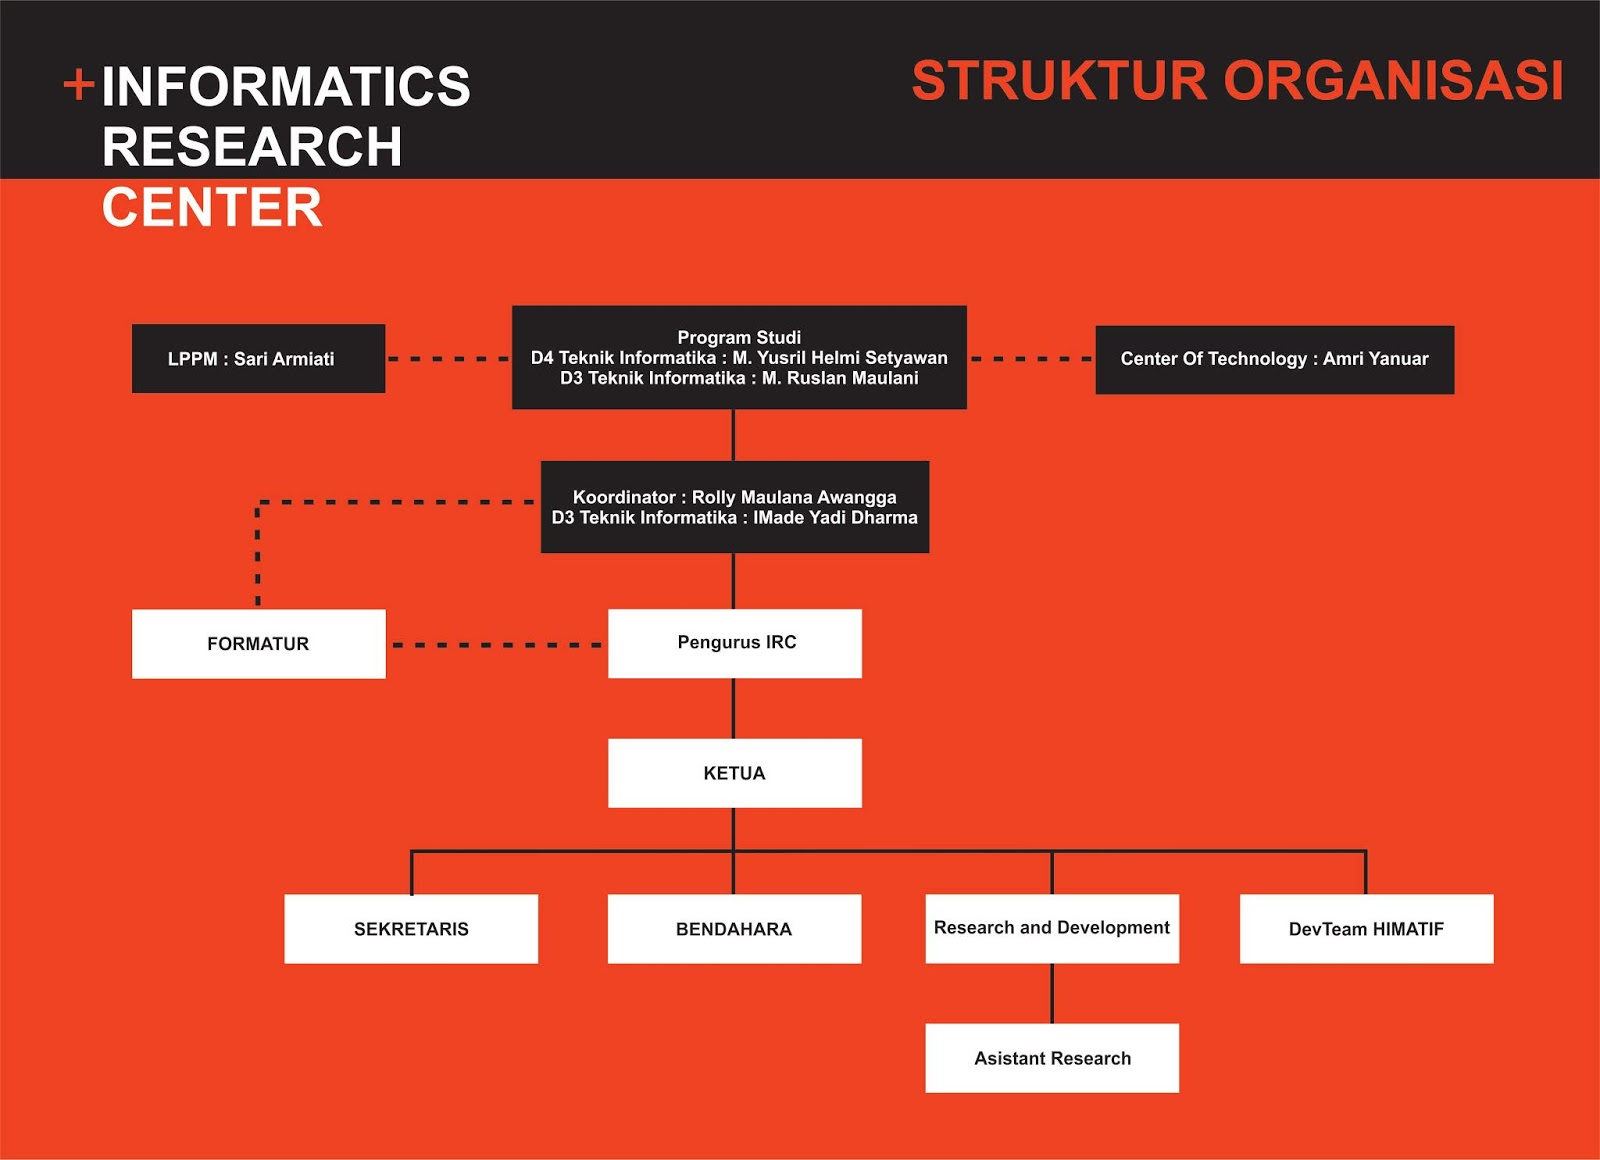
\includegraphics[scale=0.2]{figures/strukturIRC.jpg}
\caption{IRC Organizational Structure}
\label{labelgambar3}
\end{figure}

\subsection{Job Description of case study}
Job description that of the IRC are as follows:
\begin{enumerate}
    \item EEG data processing
    \item Research Electroencephalogram (EEG) 
\end{enumerate}

\section{Data description source}
\subsection{Description Participants Internship Job Type I}
In this internship activities, Internship program authors conducted the first in IRC and positions as an internship as a researcher where the function of the researcher is researching IRC.
\par
Existing jobs at the researcher, among others conduct research on Electroencephalogram on brain waves.
\subsection{Scope Internship I}
In this internship, program writers are in a division researcher to examine EEG. In EEG study, the authors conducted a development section is standard or abnormal signal detection on the EEG signal.
\subsection{Responsibilities of Participants Internship I}
The responsibility of the author during this internship program, among others, can undertake the task given by an external supervisor, take the development of problems that occur in the EEG.
\subsection{Participants Job Description Internship How Far I}
In this internship, program author gets some work related to the development of the EEG. Work is researching drug users by users with EEG signal detection.


\chapter{Methods}

\section{Research Methodology}
\begin{figure}[h!]
\centering
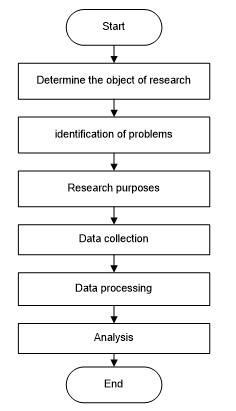
\includegraphics[scale=0.7]{figures/flowwc.PNG}
\caption{Flowchart research}
\label{labelgambar4}
\end{figure}

\section{Method Description}
Stages (groove strategies) the researchers used in the analysis of EEG data is as follows:

\begin{enumerate}
    \item Determine the object of research.
    \par
   Determine what object will be investigated in the research activity. Some things need to be understood to determine and construct an object of research in a research method, which relates to the purpose of research, besides that, each object of research and what criteria can be used as the purpose of the research that we do[19], in this study I had the opportunity to examine a drug user in the brain of the drug user and in this study I assessed brain waves by using EEG (Electrocardiograph) determination of brain waves to be explained here based on the amplitude of certain objects
   
    \item Identification of problems
    \par
   Problem identification is the process and result of problem recognition. In other words, problem identification is one of the research processes which is arguably the most important among other procedures. Research problems will determine the quality of research, in this step the researcher can find out more, can by conducting observations, reading the literature identifies one aspect that has been determined with the relevant environment (drug users) that is relevant.\cite{chappell2018constructing}
   
    \item Research purposes
    \par
    The purpose of this study was to obtain a formula for the results of research through the process of searching, discovering, developing, and testing surveys conducted.In this phase the researchers aimed to process the data. The purpose of this study could provide a basis for further developing research that builds evidence about brain waves of drug users\cite{chappell2018constructing}

    \item Data collection
    \par
    Data collection was conducted to obtain information required in achieving the goal of research being done. Before attending the study, the researchers usually have had a notion based on the theory that he used, each study had a data collection process that is different depending on the type of research that is being researched
    
    \item Data processing
    \par
 The image below is the process of processing data using Wavelet. the processed data is the data obtained from the EEG signal recording process, Bandpass Filter and ICA data after processing from Matlab. At this stage of data processing researchers conduct data processing on someone who is a drug user, at this stage researchers will also get the results of data processing in the form of amplitude..	
  
  \begin{figure}[h!]
\centering
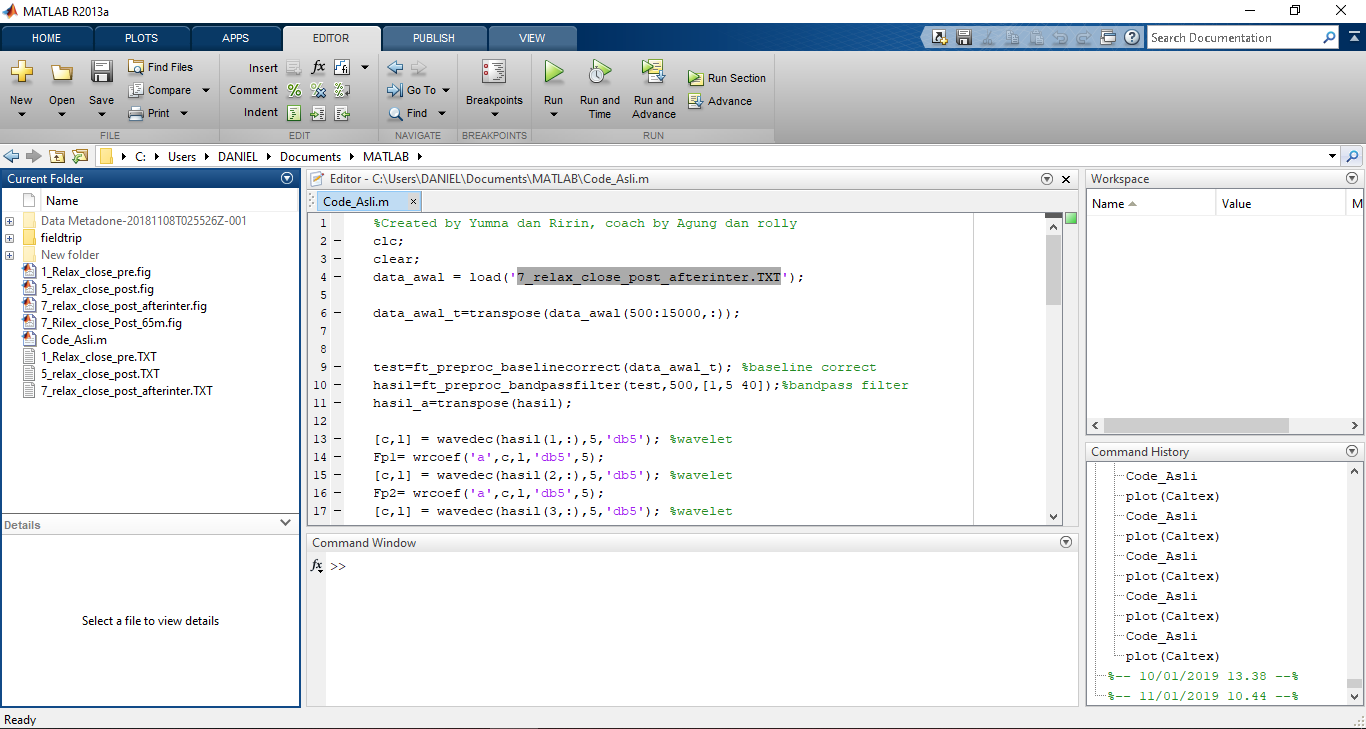
\includegraphics[scale=0.3]{figures/proses1.PNG}
\caption{Data Processing}
\label{labelgambar5}
\end{figure}
  
    \item results
    \par
    The results of processing the data researchers obtain information that has been processed beforehand and researchers get the results of brain waves of drug users.
    
\end{enumerate}


\chapter{Experiment and Result}
\section{Experiment}
\subsection{Tools Used}
To process the EEG signal, there are a wide variety of devices that can be used in EEG data processing, among others:

\subsubsection{EEG amplifier Mitsar -202 and WinEEG}
For the EEG signal acquisition phase in this study, the hardware used is an EEG amplifier Mitsar-202 32 channels. Display devices of this amplifier can be observed in Figure 5.1
\begin{figure}[h!]
\centering
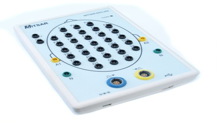
\includegraphics[scale=0.5]{figures/51.PNG}
\caption{EEG amplifier system Mitsar-202}
\label{labelgambar5}
\end{figure}

\par
To record EEG signals using this amplifier, the amplifier device is connected to a PC using USB. Furthermore, speakers WinEEG operated via software on the PC. WinEEG program display can be observed in Figure 5.2.
\begin{figure}[h!]
\centering
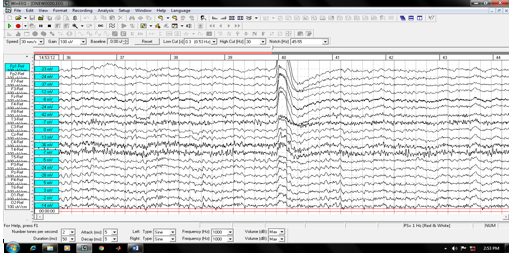
\includegraphics[scale=0.5]{figures/52.PNG}
\caption{Display software WinEEG}
\label{labelgambar6}
\end{figure}

\subsubsection{ Electro-Cap}
\par
Electro-Cap a hat-shaped device that serves to facilitate the placement of EEG electrodes. This device consists of some lead electrodes connected to an amplifier via adapters (Electro-Cap International, Inc., 2015). Views Electro-Cap can be observed in Figure 5.3
\begin{figure}[h!]
\centering
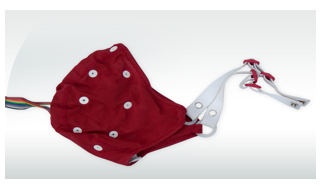
\includegraphics[scale=0.5]{figures/53.PNG}
\caption{Electro-Cap}
\label{labelgambar7}
\end{figure}

\subsubsection{MATLAB}
\par
MATLAB is a high-level programming language for applications in various fields, such as numeric computation, analysis, and data visualization software and algorithm development, and design of the model system. (MathWorks, 2017) MATLAB toolbox is complemented by a wide range to support specific tasks, either developed directly by MathWorks and third parties. In this study, the toolkit is used field trip.

\par
The field trip is an open source software for EEG analysis, magnetoencephalography (MEG), electrophysiological data and more. The software supports a variety of functions for the study of EEG as a pre-processing of data, ERP analysis, classification, and others. Here is a preview of the software is MATLAB icon 2017.
\begin{figure}[h!]
\centering

\includegraphics[scale=0.6]{figures/54.PNG}
\caption{The initial view Matlab}
\label{labelgambar8}
\end{figure}

\section{Data Processing}
\subsection{Pre-Processing}
\par
Pre-processing is beginning the process of signal processing that consists of raw, and bandpass filter and Brain Mapping. Such procedures would improve the signal by removing artifacts, and present signals are more easily analyzed.

\subsubsection{raw Data}
\par
To record EEG signals using this amplifier, the amplifier device is connected to a PC using USB. Furthermore, speakers WinEEG operated via software on the PC. WinEEG program display can be observed in Figure 5.5
\begin{figure}[h!]
\centering
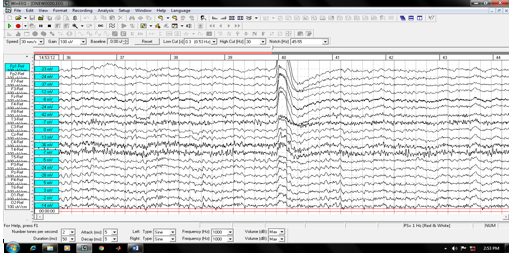
\includegraphics[scale=0.6]{figures/52.PNG}
\caption{Example of Display Raw Data Subject}
\label{labelgambar9}
\end{figure}

\par
Raw Data is the raw data that has not been treated at all. Wave signal is still very rough and irregular caused by artifacts in the message. Raw EEG signal data on each channel can be seen
\begin{figure}[h!]
\centering
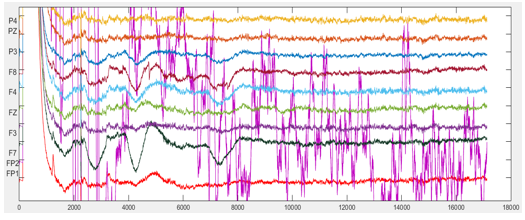
\includegraphics[scale=0.6]{figures/55.PNG}
\caption{Example of Display Raw Data Subject}
\label{labelgambar10}
\end{figure}

\subsubsection{bandpass Filter}
\par
Bandpass filter with a frequency range of 3 Hz to 30 Hz is used to the raw data. Bandpass filters on the EEG signals are shown in Figure 5.6
\begin{figure}[h!]
\centering
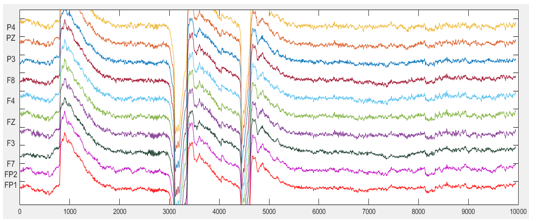
\includegraphics[scale=0.6]{figures/56.PNG}
\caption{Display EEG data after Bandpass Filter}
\label{labelgambar10}
\end{figure}

\subsection{Data Processing Using Wavelet}
\par
The wavelet transform is a method of signal processing requires the workings resemble signal analysis using the Fourier transform by splitting the signal to be analyzed into several parts. The difference, tell the Fourier transform of a signal frequency information, but not with the timing information but the wavelet transform signal in the time domain into signals in the time and frequency, in this case, is formed into an area of translation and scale. Translation (reading) is a form of transformation from the time domain translation associated with the location of the window function, where window be moved along the incoming signal. Scale (scale) is a form of transformation of frequency, where the value scales inversely proportional to the frequency value.

\section{Result}
\par
At this stage, to see the most dominant brain activity. Here is a scene Wavelet application configuration and the results of Brain Mapping one subject

\begin{enumerate}
 \item Result Rilex Close Pre
     \begin{figure}[h!]
\centering
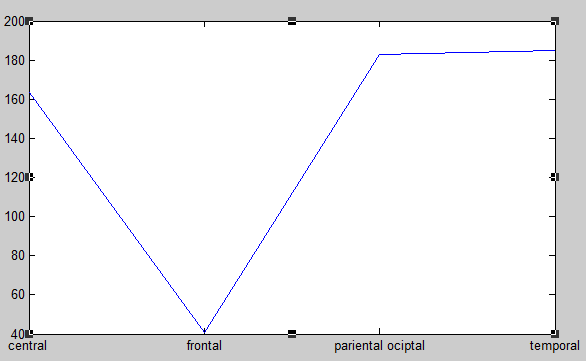
\includegraphics[scale=0.6]{figures/hasil1.PNG}
\caption{The Brain Sigbal Rilex Close Pre}
\label{labelgambar5}
\end{figure}

\par
picture Result Rilex Close Pre above is the result of processing data using wavelets. the graph above is the result of recording subject 1 data in relaxed and closed eyes. in this condition, the subject is told to close his eyes and not think of anything. after recording and processing data, the subject's brain condition can be seen based on the picture above. the result, the central subject brain condition is 160Hz, Frontal 40Hz and the ociptal Pariental is at 180Hz

\item Result Rilex Close Post after 4 minutes
\begin{figure}[h!]
\centering
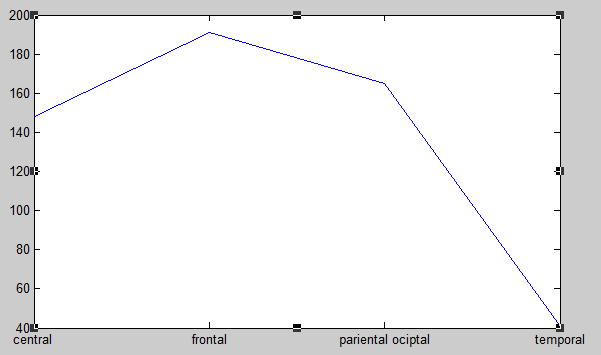
\includegraphics[scale=0.6]{figures/hasil2.PNG}
\caption{The brain signals Rilex Close Post after 4 minutes}
\label{labelgambar12}
\end{figure}

\par
picture Result Rilex Close Post after 4 minutes above is the result of processing data using wavelets. The graph above is the result of recording subject 1 data after the administration of methadone for 4 minutes. in this condition, data in colleagues used WinEEG on subjects who had been given methadone. after recording and processing data, the subject's brain condition can be seen based on the picture above. As a result, the central subject brain condition is 150Hz, Frontal 190Hz, Ociptal Pariental is at 160Hz and temporally 40Hz
\item Result Rilex close post after 65 minutes
\begin{figure}[h!]
\centering
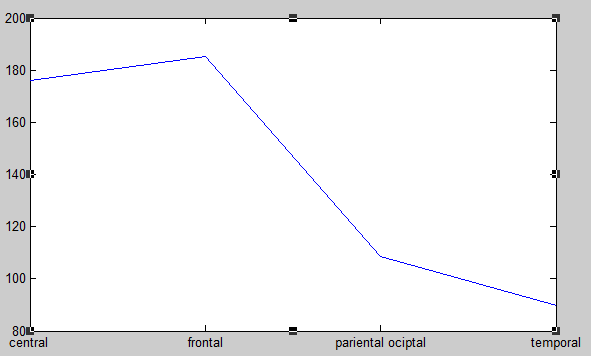
\includegraphics[scale=0.6]{figures/hasil3.PNG}
\caption{Rilex Close Post after 65 minutes}
\label{labelgambar13}
\end{figure}

\par
picture Result Rilex close post after 65 minutes above is the result of processing data using wavelets. the graph above is the result of recording subject 1 data after giving methadone for 65 minutes. in this condition, data in colleagues used WinEEG on subjects who had been given methadone. after recording and processing data, the subject's brain condition can be seen based on the picture above. As a result, the central subject brain condition is 160Hz, Frontal 200Hz, and the ociptal Pariental is at 110Hz.
   
\end{enumerate}

    
\chapter{Conclusion}
\section{Conclussion of Problems}
\par
        By paying attention to data processing and analysis in the previous chapter it can be concluded that wavelet is a signal processing method that requires work methods similar to Fourier signal decomposition can be used to identify how a person's brain is a drug user or not a drug user. 
        
\section{Conclusion of Method}
\par
The conclusions obtained in this research method are where the researcher determines the method used to process the data from the object determined by the research will determine the quality of the research. In this step the researcher can find out more, by observing, reading the literature identifying one predetermined aspect with relevant environmental (drug users) relevan.

\section{Conclusion of Experiment}
\par
In this study, eeg signals that have been recorded using WINEEG and analysis using WAVELET can be concluded that the condition of the otas of the person being studied can be observed. Observations made by comparing the results of the subject's brain data record before and after being given a stimulus. This analysis also shows large variations due to drugs or methadone. Therefore, the use of the proposed method, the assessment of the brain condition of drug users using WAVELET, the brain condition of drug users and the identification of efficient EEG signals can help in research.
\chapter{Discussion}

\par
       Methadone is a type of synthetic opioid drug, used as an analgesic and for treating addiction from users of the opioid group, such as heroin, morphine, and codeine. But improper use can also have a negative impact on health. Although methadone is very necessary for medical care and services, especially drug addicts, if it is misused or used is not in accordance with the standard of care, especially if accompanied by illicit circulation, it will have a very detrimental effect on individuals or society, Electroencephalogram (EEG) is an activity to record the electrical activity of brain neurons. Using EEG, the condition of relaxing or not drug users can be observed. EEG signals are widely used to detect brain disorders in the world of health. However, EEG signals are not made to be ready to detect brain abnormalities automatically. Therefore, the characteristics of the EEG signal are safe.Simultaneous EEG modulation of the volume of BOLD activity from the target brain region and investigation of electrophysiological activity related to the results of objects using illegal drugs will show human brain waves.
    
\par
    The conclusions obtained in this research method are where the researcher determinesthe method used to process the data from the object determined by the research willdetermine the quality of the research.  In this step the researcher can find out more, byobserving, reading the literature identifying one predetermined aspect with relevantenvironmental (drug users) relevan.
    
\par
    In this study, eeg signals that have been recorded using WINEEG and analysis usingWAVELET can be concluded that the condition of the otas of the person being studiedcan be observed.  Observations made by comparing the results of the subject’s braindata record before and after being given a stimulus.  This analysis also shows largevariations due to drugs or methadone.  Therefore, the use of the proposed method, theassessment of the brain condition of drug users using WAVELET, the brain conditionof drug users and the identification of efficient EEG signals can help in research

%now enable appendix numbering format and include any appendices
\appendix
\include{section/appendixA}
\include{section/appendixB}
\include{section/appendixC}
\include{section/appendixD}
\include{section/appendixE}
\include{section/appendixF}


%next line adds the Bibliography to the contents page
\addcontentsline{toc}{chapter}{Bibliography}
%uncomment next line to change bibliography name to references
%\renewcommand{\bibname}{References}
\bibliography{references}        %use a bibtex bibliography file refs.bib
\bibliographystyle{plain}  %use the plain bibliography style

\end{document}

